\chapter{Methods}\label{chapter:method}

{ \color{red}

    about 10-30 pages (rather more I guess)

    \begin{itemize}
        \item (1/3 of thesis)
        \item start with a theoretical approach, describe the developed system/algorithm/method from a high-level point of view,
        \item go ahead in presenting your developments in more detail
        \item make sure to not refer to results section too much. rather leave info out if it cannot explained well without looking at the results
    \end{itemize}
}

\section{Causal Model}
The core aspect of our analysis is the combination of causal methods for data generation and ground-truth feature attribution. 
The main process includes a hyperparameter such as the later discussed coupling ratio $\rho$ which one can intervene on, trained models and their resulting predictions and explanations generated for single instances using a model and its output. 
Within this greater structure, a subprocess constructs the image dataset with a structural causal model, taking only $\rho$ as an input. While $\rho$ stays fixed for each model to be trained, it is a causal variable in the overarching structure. This way we create an array of causally generated datasets whose constitution only differs by this one variable. 

\subsection{Data Generating Causal Model}
For the most exact comparison of attribution between a model and its explanation it is imperative to know the ground truth of the training data. A structural causal model (SCM) can define variables and the \textit{independent} mechanisms with which they interact precisely. We want to define an SCM that closely mirrors image generation processes as they happen in realistic scenarios. 
Explicitly using a generating SCM has previously been done to create or test new attribution methods \cite{Parafita2019, Wilming2023, Clark2023, Goyal2019, Reimers2019, Reimers2020}. A few other works evaluating XAI methods with a known ground truth have implicitly used structures akin to an SCM without defining it in causal language \cite{Kim2018, Yang2019, Arras2022}. 

The causal graph and its structural assignments used for our experiment are defined as follows: 
\begin{equation}
\label{eq:scm}
\begin{aligned}[c]
&G:=\eta^g \notag \\ 
&N_w:=\eta^w  \notag \\ 
&N_s:=\eta^s \notag \\ 
&N_x:=\eta^x  \notag \\ 
&W:=(\rho * G + (1-\rho)* N_w) \geq 0.5 \notag \\ 
&S:=(\rho * G + (1-\rho)* N_s) \geq 0.5 \notag \\ 
&Z:= \eta^z \\ 
& \mathcal{X} = W + f_{image}(S, Z) + N_{x} \\
\end{aligned}
\begin{aligned}[c]
& \mathrm{with} \  \eta^g \sim \mathcal{N}(0.5,0.02) && \notag \\ 
& \mathrm{with} \  \eta^w \sim \mathcal{N}(0.5,0.1) && \notag \\ 
& \mathrm{with} \  \eta^s \sim \mathcal{N}(0.5,0.1) && \notag \\ 
& \mathrm{with} \  \eta^x \sim \mathcal{N}(0,0.05) && \notag \\ 
\\
\\
& \mathrm{with} \  \eta^z \sim \mathcal{U}(0,245760) && \notag \\ 
\\
\end{aligned}
\end{equation}

\begin{figure}[t!]
    \centering
    \includegraphics[width=0.9\textwidth]{pics/generating_scm.png}
    \caption[Data Generating SCM]{Data Generating Structural causal model.
        $\rho$ is not explicitly visible in the SCM. It determines the signal-to-noise ratio between the confounding $G$ and the noise variables $N_w$ and $N_s$. The noise terms of $Z$ and $G$ are not shown explicitly.}
    \label{fig:generating_scm}
\end{figure}

The SCM as seen in \cref{fig:generating_scm} and \cref{eq:scm} serves as a ground truth for our experiment. It is mostly an additive model using Gaussian distributions for the noise terms, except for $Z$ which uniformly at random selects other image generating factors like rotation, scale and position of the shape. Also the function $f_{image}$ generating the images out of the latent factors and the shape is not further specified.

The meta-variable $\rho$ adjusts how much information is shared between the true class information (shape), which we name \textit{core feature} following \cite{Singla2022} and the watermark or \textit{spurious feature} through a shared common ancestor named \textit{generator} $G$. For each model coupling ratio $\rho$ is fixed, to later enable a comparison between models trained with different coupling ratios. \\

A second parameter which we keep fixed for all experiments, determines how frequent the spurious feature is in the data. We set this parameter which can be seen as the \textit{prevalence} to 0.5, so that just as many images have a watermark as not. Notably, when $\rho$ is 1 this means that all ellipses will have the watermark and no rectangle will and when $\rho$ is zero there is no correlation of watermark and shape. \\

It is important to note that this particular SCM is just one of many possible ways to model how spurious features might interact with core features. It attempts to follow the logic of how images are generated or selected in real datasets. Here, it particularly looks at pathways for the generation of \textit{Clever-Hans} or \textit{watermark} features, often present in image datasets \cite{Lapuschkin2019}. As visible in \cref{fig:equivalent_scm} different causal models can produce an equivalent distribution of the two latent factors in question (watermark and shape). One can think of more variations of SCMs which are able to produce the same correlation, so the choice of using the confounder version as in \cref{fig:generating_scm} is mainly due to its ease of implementation. It also lends itself best to the Clever-Hans task, because in this SCM there is no real causal effect between the core and spurious feature. It would therefore be ideal for the a neural network to ignore the spurious feature completely. Without assumptions about the generating mechanism though, the confounder case is not identifiable, i.e. distinguishable from $W \rightarrow G \rightarrow S$ and $S \rightarrow G \rightarrow W$ because it is Markov equivalent to those scenarios. 
Although the presented collider case (\cref{fig:equivalent_scm}\textbf{a}) is theoretically distinguishable from the confounder case (\textbf{b}), one can not hope that a network which only has access to the intervened on (selected) data will recover this. 

The idea of investigating the effect of a coupling ratio $\rho$ was inspired by Clark et al. \cite{Clark2023}, who also used a \textit{signal-to-noise} ratio in their generating model. Instead of a confounding model their learned data instances are colliders of the label and a suppressor variable similar to \cref{fig:equivalent_scm} \textbf{a}. In their experiments the expected explanation importance of this suppressor feature therefore ought to be zero, as long as the collider is not intervened on. We contest this assumption, as it is not clear whether a neural network does not implicitly conditions on this collider (which is the image set), therefore introducing correlation between the parent components through a selection bias. We disagree with their statement that a good explanation method ought to not attribute any importance to such suppressor variables. This is, as Nauta et al. \cite{Nauta2023} put it, a case of conflating external \textit{coherence} i.e. ''agreement with human rationales'' \cite{Atanasova2020} with \textit{correctness} towards the model. As we are not aware of any explicit way in which deep neural networks differentiate between a suppressor or confounder variable, it is wrong to expect an explanation to explain something the model cannot even conceptualize. 

The direction of causal links for image classification is as can be seen from this example highly debatable and shall not be the focus of this work. Whether the selection of the AI researcher reducing costs with free images resulted in classes being polluted with watermarks (\cref{fig:equivalent_scm}\textbf{a}), or whether a scientist marked x-rays with their diagnosis (\cref{fig:equivalent_scm}\textbf{b}) seems to not be distinguishable for ML models. 
Instead, we only want to find to what degree a neural network learns, and then attribution method explains the distribution generated by a particular SCM.

This first experiment is supposed to test whether the framework we apply is in principle reasonable and to establish a baseline for how feature importance behaves. To further illuminate its applicability we look at other SCMs with different datasets in the results (\cref{chapter:results}). Specifically, we want to compare the result of this SCM for a scenario where the spurious feature is spatially separated from the core feature to one where they overlap. 
If time allows, it would also be interesting to see if the suppressor variable model produces results differing from the confounded case.

\begin{figure}[t!]
    \centering
    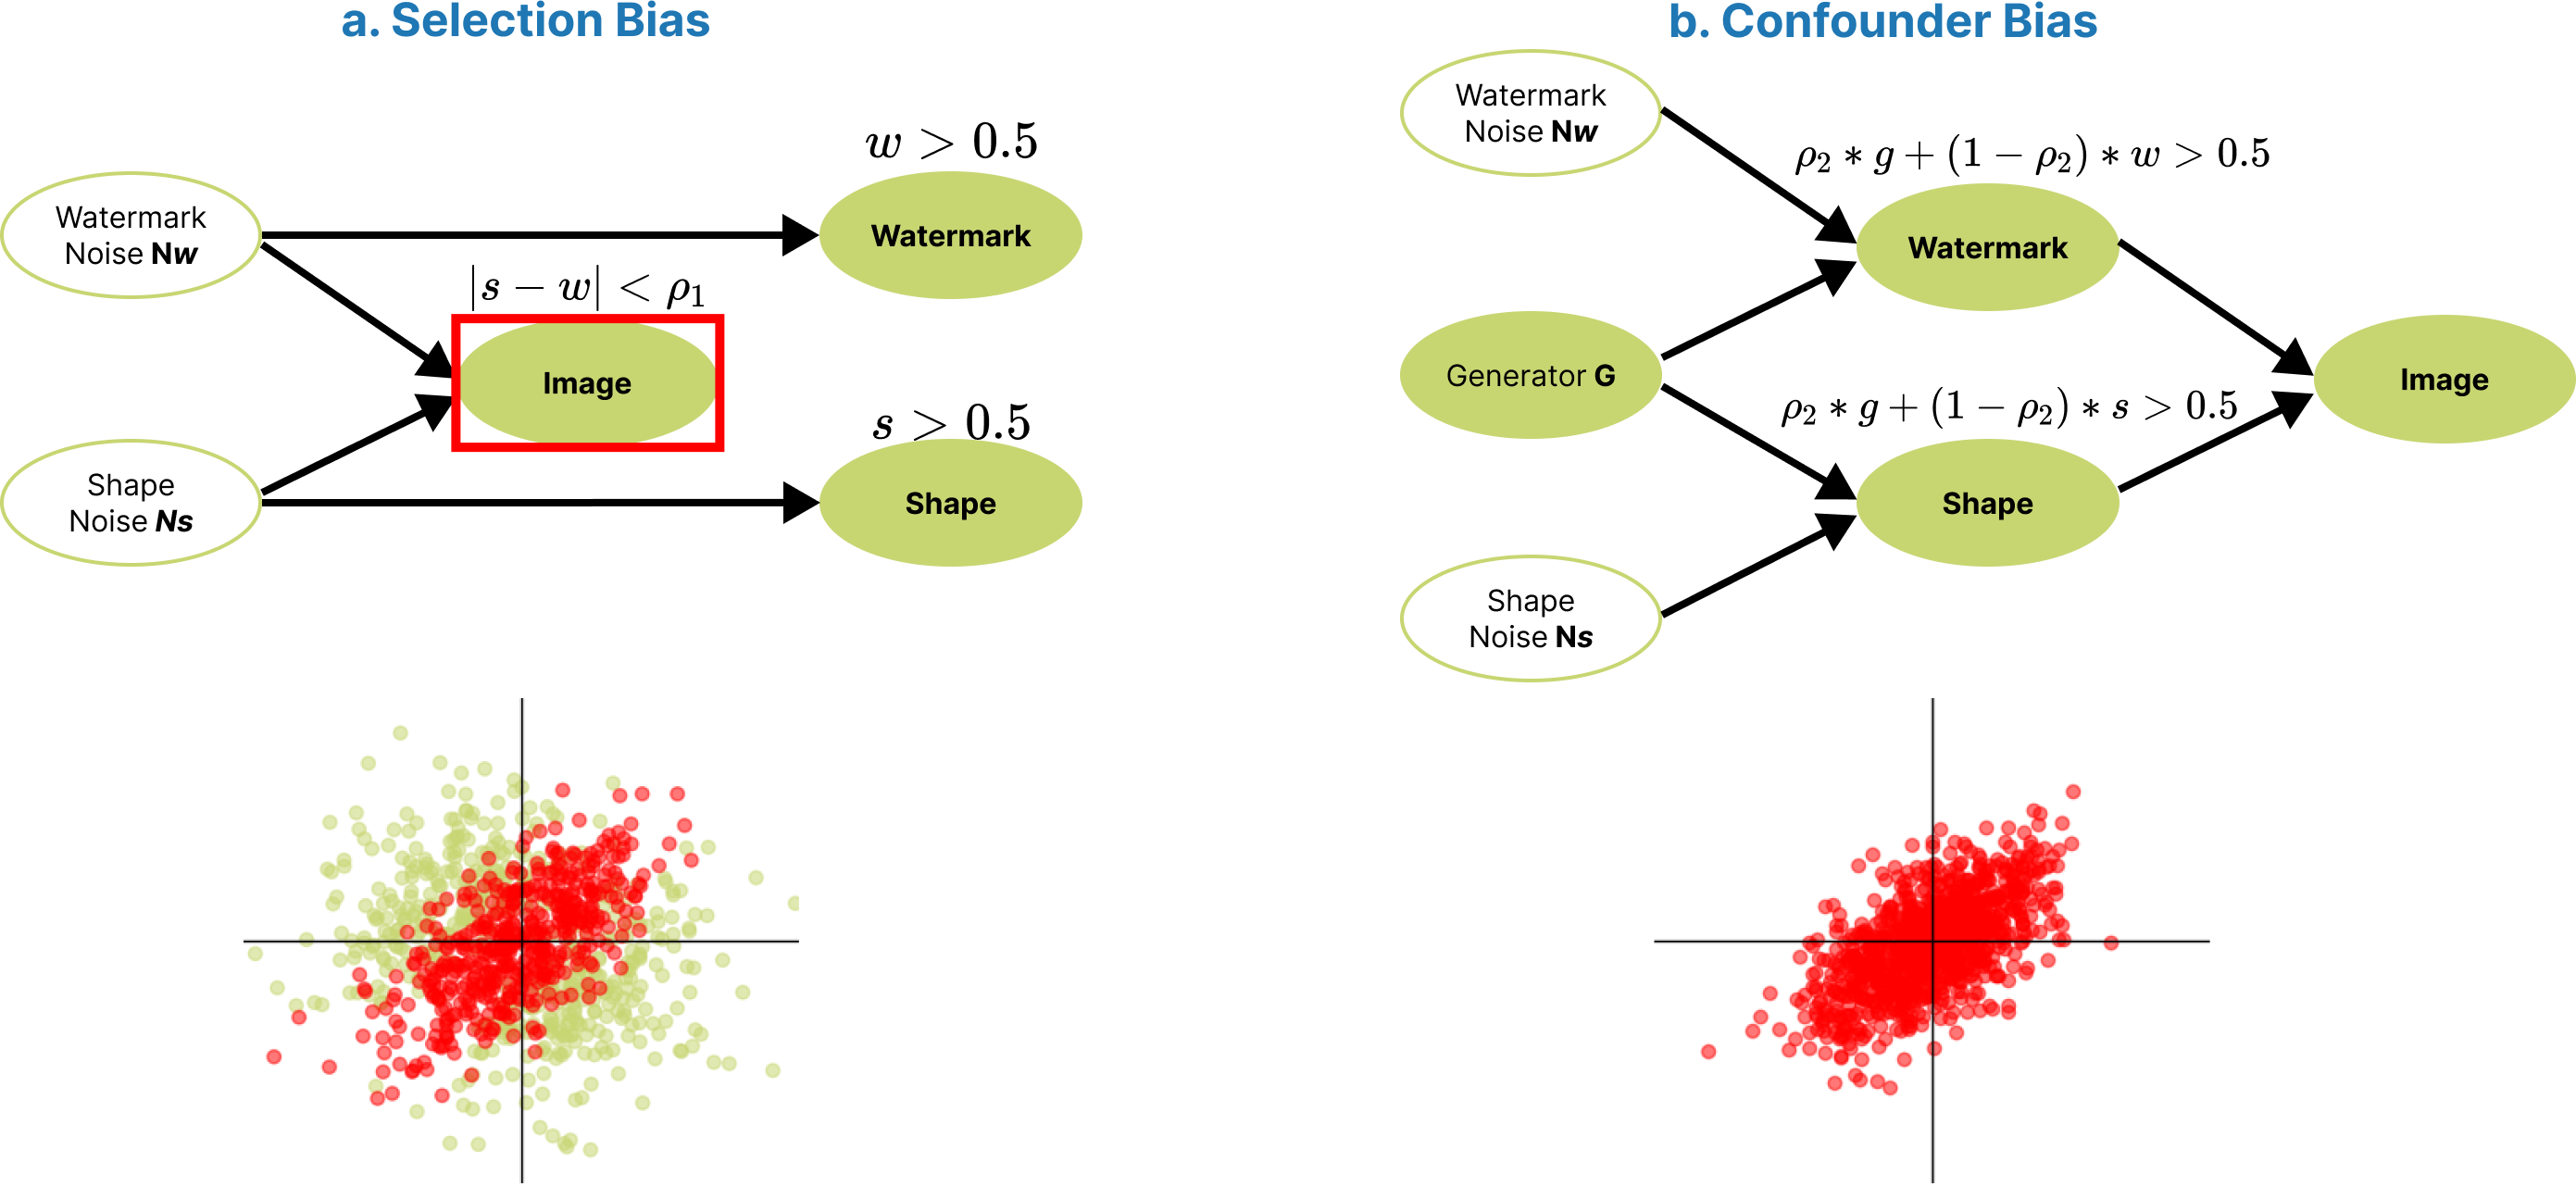
\includegraphics[width=0.8\textwidth]{pics/equivalent_scm.png}
    \caption[Selection vs. Confounder Bias]{SCMs typically found in image datasets.
    \textbf{a.} Selection Bias \textit{(researcher chooses images from free online collection with watermarks)}
    \textbf{b.} Confounder Bias \textit{(e.g. scientist marks positive x-ray scans with sign)}}
    \label{fig:equivalent_scm}
\end{figure}

\subsection{Explanation Generating Model}
The data generation causal model is part of the model which generates predictions and explanations.
This model is defined in a similar way to the \textit{explanation generating process (EGP)} in Karimi et al. \cite{Karimi2023}.
Ratio $\rho$ is a meta-variable of our image generation process in a similar sense to how hyperparameters are defined for the training there. While \cref{fig:generating_scm} depicts the data generating causal model (DGCM) of the training dataset in more detail, \cref{fig:egp} shows how this is embedded into the mechanism of generating explanations. 

\begin{figure}[t!]
    \centering
    \tikzset{%
        neuron/.style={
            ellipse,
            draw,
            minimum height=8mm,
            },
        arrows={[scale=1.2, angle 60]}
    }
    \begin{tikzpicture}[]
    % generating model:
        \node [neuron]  (r) at (0,4) {$\rho$};
        \node [neuron]  (rs) at (3,3) {seed};
        \node [neuron]  (scm) at (2,4) {DGCM};
        \node [neuron]  (w) at (5,4) {weights};
        \node [neuron]  (x) at (5,2) {$\mathcal{X}$};
        \node [neuron]  (p) at (7,3) {$Y$};
        \node [neuron]  (e) at (9,2) {$E$};
        
        \draw[->] (r) -- (scm);
        \draw[->] (scm) -- (w);
        \draw[->] (rs) -- (w);
        \draw[->] (w) -- (p);
        \draw[->] (x) -- (p);
        \draw[->, bend left=40] (w) to (e);
        \draw[->, bend right=20] (x) to (e);
        \draw[->] (p) -- (e);
    \end{tikzpicture}
    \caption[Explanation Generation Process (EGP)]{Explanation Generation Process \textit{EGP}}
    \label{fig:egp}
\end{figure}

\subsection{Watermark Benchmark Dataset W-dSprites}\label{section:causal_model}
Although this thesis is not the first work to use a toy dataset with known generating factors to evaluate attribution methods, we aim to find a new dataset which is as simple as possible and yet mirrors the main workings of a realistic computer vision problem. For this we adapted the dSprites dataset \cite{dsprites17} by adding small watermarks in the shape of '\textit{w}'s to some images. The dSprites dataset was originally constructed as a means for testing the degree of disentanglement a machine learning model has achieved. It contains images with rectangles, ellipses or hearts in varying positions, scales and rotations. To simplify the task more we only use the rectangle and ellipse class for our experiment. Another motive is that in a binary classification task positive and negative relevance might be used in varying strategies for prediction. In theory this could make the class-insensitivity studied by Sixt et al. \cite{Sixt2020} visible or counteract it. Further details can be found in the appendix \cref{appendix:dsprites}.

\begin{figure}[t!]
    \centering
    \includegraphics[width=0.6\textwidth]{pics/dsprites_examples.png}
    \caption[Example Images W-dSprites]{First row: images from the original dSprites dataset, second row: images from the W-dSprites dataset with small \textit{w} as a watermark on some images in random positions at the edge of the image and Gaussian noise added.}
    \label{fig:dsprites_examples}
\end{figure}

\section{Generating Explanations with Concept Relevance Propagation}\label{section:explanations_with_crp}
The previously described causal framework can be applied to a multitude of explanation methods as it is principally model- and method-agnostic. However we limit our analysis to CRP and interpretation techniques constructed with CRP. This is mostly due to the time limitations of a master thesis, but also because its authors specifically claim in their paper to be able to identify relative importance using CRP. 
Producing explanations using concept relevance propagation requires decisions on the backpropagation rule(s), on the conditioning sets and further hyperparameters. 
We follow the recommendations and default settings of CRP's authors \cite{Achtibat2022, Achtibat2023} and best practices \cite{Kohlbrenner2020} as closely as possible.
For the backpropagation we apply the $LRP_{\varepsilon -z^+- b^-}$ - rule as recommended by \cite{Kohlbrenner2020}. Due to the simplicity of our CNN model no more model canonization steps need to be applied. See \cref{appendix:lrprules} for further technical details. 

\begin{figure}[t!]
    \centering
    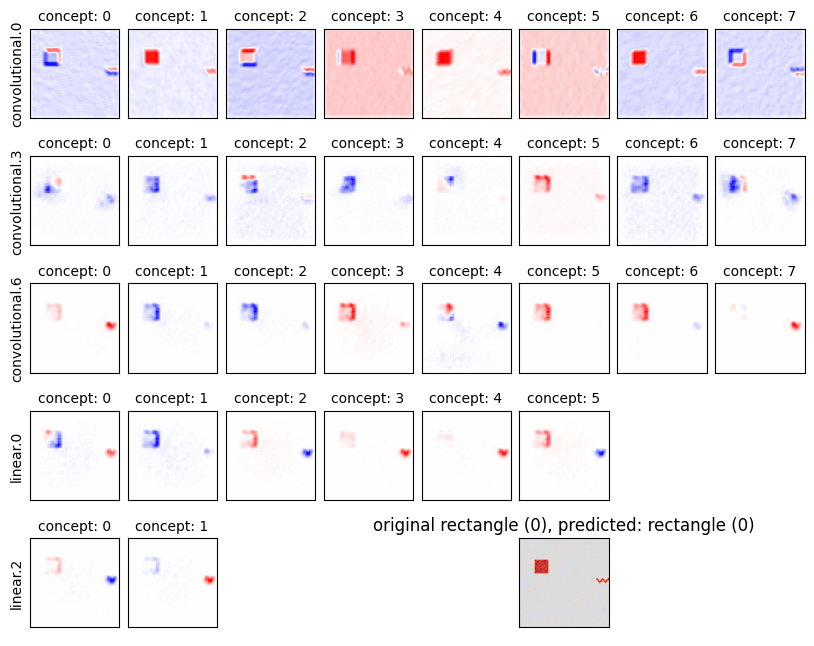
\includegraphics[width=0.8\textwidth]{thesis_latex_template/pics/conditional_heatmaps.png}
    \caption[Comparing Attribution Maps of Layers]{Concept-conditional heatmaps for one example image. Note the Sobel-filter-like attributions in earlier layers and the more combined attributions of watermark and shape in later layers.}
    \label{fig:cc_heatmaps}
\end{figure}

% Maybe say something about how concept atlas and hierarchical attribution graphs can help us decide which concepts seem to be most disentangled (if heatmaps are indeed correct that is). THen show image below to visualize how to choose? 

%\begin{figure}[t!]
%    \centering  
%	\includegraphics[width=\textwidth]{thesis_latex_template/pics/concept_atlas_all.png}
%    \caption[Concept Atlas and Hierarchical Attribution Graph]{Concept Atlas and Hierarchical Attribution Graph for an image in our dataset, looking at how negative or positive relevance flows from the output through each layer. Here, concept 0 and 7 seem to redundantly encode the right half of the ellipse, while 5 and 6 encode the watermark in the last convolutional layer. }
%    \label{fig:attr_graph}
%\end{figure}

Principally, neurons in every layer of a model can be conditioned on using the CRP-approach. However, the resulting attribution maps are not necessarily depicting disentangled \textit{and} abstract enough concepts. When looking at \textit{concept-conditional} attribution maps from the earlier layers, one will likely see low-level features akin to Sobel-filter. In the late, fully connected layers before the output the previously disentangled concepts might get mixed together again for the final decision. In \cref{fig:cc_heatmaps} an example shows the tendency from trivial to abstract \textit{concepts}. 
According to \cite{Dreyer2023a} referring to \cite{Zeiler2013} the \textit{last convolutional layer} is ''most likely representing disentangled representation''. For comparison we investigate both the last convolutional and the first fully connected layer of the model. It is not entirely clear whether the extremely small size of our model hinders a transfer of the results to realistic scenarios. Yet, training significantly larger models would have been too computationally expensive for this principled approach, requiring many trained models.\\

In the following we will reiterate the steps necessary to produce the different components of CRP-explanations:

\subsubsection{Concept-Conditional Attribution Maps and Relevance for Prediction}
The concept-conditional backpropagation rule described in \cref{section:crp_background} can be applied to arbitrary sets of neurons (i.e. filters) $\theta$. In our scenario we create class-specific attribution maps conditioned on each individual neuron (termed concept $c$) in the selected layer. For this, we use the output for the ellipse class as the initialization for relevance, keep all other layers untouched and then mask out the desired neurons $c$ relevance in the layer $\ell$: 
\begin{equation}
    R^{\ell}(\mathrm{x} |\theta_{c}) = \sum_{i} R_i^{\ell}(\mathrm{x} |\{y=1\} \cup \theta_{\ell} = \{c\})
\end{equation}
Here $i$ represent all relevances in lower layers that are a part of the concept $c$ and not masked out. 
To yield the attribution map, the importance is backpropagated through all layers till the input layer $\ell = 1$ and not summed per input feature $i$, producing individual relevances  termed $R_{i}^{1}(\mathrm{x} |\theta_{c})$. In the following we will refer to this concept-conditional attribution map as $\mathcal{A}_c(\mathrm{x})$ and the class specific relevance of concept $c$ as $R_c^{\ell}(\mathrm{x})$. Due to the \textit{conservation laws} that CRP inherits from LRP (Equation 7 \cite{Achtibat2022}) the relevances $R_c^{\ell}$ within one layer can be interpreted as the \textit{percentage} of importance going through concept $c$. To enable this view also for out-of-distribution samples the authors recommend normalizing the relevances to sum to 1:
\begin{align}
    R^{\ell}_{norm}(\mathrm{x} |\theta_{c}) = \frac{R^{\ell}(\mathrm{x} |\theta_{c}) }{\sum_k |R_k^{\ell}(\mathrm{x} |\theta_{c})|}
\end{align}

\subsubsection{Local Concept Importance}
To find out how much a certain region contributes to the overall prediction but also which concepts are most highly activated within that region, the authors propose local concept importance. 
This method simply masks out the desired region, i.e. the input features, within the concept-conditional attribution map and sums the relevance within that mask. 

\begin{align}\label{eq:local_importance}
    R_{B}^{\ell}(\mathrm{x} | \theta_c) = \sum_{(p,q) \in B} R_{p,q}^{\ell}(\mathrm{x} | \theta_c)
\end{align}
Again, for readability we from now on refer to this local concept importance in a region $B$ as $R_B$

\subsubsection{Relevance Maximization}
As described in the background \cref{section:crp_background}, CRPs authors also use concept-conditional relevance to create prototypical reference sets of each concept. In a human subject study \cite{Achtibat2023} they find this method to be useful for the identification of Clever-Hans artifacts where only using heatmaps fails. We therefore aim to include this technique into our analysis. There is no straight-forward way to quantify how much images encode a concept, but we try the following approach: If a (set of) neurons indeed encodes a spurious feature, this feature should be common in the given reference set, while other features should differ. 

\section{Data Ground Truth Correlation $m_0$}
The goal of this analysis it to gather information on how a known coupling ratio of two features interacts with their importance to the model and their explained importance. 
Measure $m_0 = \rho$ is the correlation between the shape and spurious feature in our data generating model. When $\rho$ is 0, the features are not associated at all, when it is 1 they correlate perfectly. Conceived as a \textit{signal-to-noise} ratio between the correlated and uncorrelated parts of $S$ and $W$, it can directly be used as a measure of the coupling of spurious (watermark) and core (shape) feature. However the data generating process introduces a small modification due to the binarization of the variables $W$ and $S$. It might therefore be more insightful to look at the actual correlation of the features in the generated data distribution as a ground-truth. Considering that we have two binary variables their correlation can be measured using the $\phi$-coefficient. It is also called \textit{Matthews} or \textit{Yule phi} coefficient and is essentially the Pearson correlation coefficient for two binary variables:

\vspace{1em}
\begin{minipage}[t]{0.45\textwidth}
\begin{tabular}{|c|c|c|c|}
    \hline
     & y= 1 & y = 0 & total  \\  \hline
    x= 1 & $n_{11}$ & $n_{10}$ & $n_{1*}$ \\ \hline
    x= 0 & $n_{01}$ & $n_{00}$ & $n_{0*}$ \\ \hline
    total& $n_{*1}$ & $n_{*0}$ & $n$ \\ \hline
\end{tabular}
\end{minipage}%
\begin{minipage}[c]{0.45\textwidth}
\begin{align}
& \phi = \frac{n_{11} * n_{00} - n_{10}*n_{01}}{\sqrt{n_{1*}*n_{0*}*n_{*0}*n_{*1}}}
\end{align}
\end{minipage}
\vspace{1em}

Generally, we do not want and neither expect the model to perfectly reconstruct $\rho$ or the data correlation $\phi$. After all, the strength of neural networks presumably lies in recovering the truly important feature even when other, highly correlated features are present. Though some research expects explanations to give insight into the distributions of the training data to better understand how biases might occur, even if a model has apparently learned to ignore spurious features \cite{Kindermans2017}. 

\begin{figure}[t!]
    \centering
    \includegraphics[width=0.5\textwidth]{thesis_latex_template/pics/gt_m0_phi_only.png}
    \caption[Choosing measure for $m_0$]{$\rho$ plotted against $\phi$-coefficient of sampled training data distributions and against $\phi$-coefficient of $W$ and the prediction on average (for comparison the $\phi$-coefficient to shape $S$ is also reported) }
    \label{fig:finding_rho}
\end{figure}

\section{Establishing a Ground-Truth Model Feature Importance $m_1$}\label{section:gt_measure}
In contrast to realistic application scenarios our causal framework enables us to establish the ground truth importance of features for a trained model. Similar to recent work on causal attribution \cite{Goyal2019,Parafita2019,Karimi2023} the causal effect of an intervention upstream on the output of a model can be estimated in the following way:
\begin{center}
Average Causal Effect of latent factor $W$ on output $Y$ \\
\begin{equation}
\displaystyle ACE = \mathbb{E} [ Y \ | \ do(W=1) ] - \mathbb{E} [ Y \ | \ do(W=0) ] 
\end{equation}
\end{center}

The intervention on a given latent factor is straight-forward here, as our factors of interest are both binary variables (watermark and shape). Due to our knowledge of the ground truth we can condition on all other independent latent factors and feed one image with the watermark and the same image without it through the neural network. Thereby achieving a pure intervention on our $W$.  
However it is not naturally clear how to define the output of a neural network. One can either measure the average causal effect on the binary prediction or on the output layers' logits, which change in a continuous fashion.
To account for the effect of the initialization of model weights and biases on the usage of either feature, we average each measure over multiple random seeds (see \cref{fig:gt_over_seeds}).

\subsection{Prediction Flip}
Computing the \textit{Prediction Flip}, as Sixt et al. call it in their experiments \cite{Sixt2022a}, is straight forward in our example as we can control all variables. 
This binary causal effect can be estimated as the percentage of images for which the prediction changes, when the factor is changed, which in turn is equivalent to the $\phi$-coefficient between prediction $Y$ and watermark $W$ in our scenario (see proof in \cref{appendix:phi_equals_pf}). Therefore this measure is apt for the comparison with the $W,S$ correlation in the training data distribution.

We expect this variant of the model importance to only become sensitive to the spurious watermark feature $W$ for higher values of $\rho$. The reason being, that while the continuous output vector (i.e.\textit{confidence}) might already be affected by the spurious feature for weakly biased models, the prediction will only flip once the spurious feature becomes more easy to identify than the core feature. 

For better readability we will refer to an image with the watermark $\mathrm{x}_{do(W=1)}$ as $\mathrm{x}$ and the same image without the watermark $\mathrm{x}_{do(W=0)}$ as $\mathrm{x'}$ in the rest of the thesis.
\begin{align}
\displaystyle 
& PF =\frac{1}{|\mathcal{X}|} \sum_{\mathrm{x} \in \mathcal{X}} |y(\mathrm{x}) - y(\mathrm{x'}) | \\
&  \equiv \frac{|\mathrm{x}_{W=1,y=1}|*|\mathrm{x}_{W=0,y=0}| - |\mathrm{x}_{W=1,y=0}|*|\mathrm{x}_{W=0,y=1}| }
{\sqrt{|\mathrm{x}_{y=1}|*|\mathrm{x}_{y=0}|*|\mathrm{x}_{W=1}|*|\mathrm{x}_{W=0}| }}
\end{align}


\subsection{Mean Logit Change}
For the W-dSprites classification task, the output vector consists of 2 logits $y_0$ and $y_1$. The model predicts \textit{rectangle} when $y_0 > y_1$ and \textit{ellipse} otherwise. To compute the mean logit change when intervening on our spurious feature $W$, we take a sufficient amount of samples $\mathcal{X}$ from our dataset and feed them through the model. First we predict images with $W=1$ (containing a watermark) then with $W=0$. It is important to choose a reasonable distance measure between the two output vectors. \cite{Sixt2022a} and \cite{Goyal2019} use the mean absolute difference (or $L1$-norm). To enable better comparison we use the soft-max confidences as during the training process. This keeps the relative magnitudes within the sample set intact but brings it to the range $[0,1]$. Although we compute the euclidean distance for other measures for the explanations later, this is not necessary here, as for 2D vectors $D_{euclid} = \sqrt{D_{abs}}$.\\

Mean Absolute Difference:
\begin{align}\displaystyle 
& \MLC_{\rho, m}^{abs} = \frac{1}{|\mathcal{X}| * 2} \sum_{\mathrm{x} \in \mathcal{X}} 
|y_0(\mathrm{x}) -y_0(\mathrm{x'})| + |y_1(\mathrm{x}) -y_1(\mathrm{x'})| 
\end{align}

Recently, assessing the similarity of activation and relevance vectors has been done using the cosine similarity \cite{Sixt2020, Dreyer2023a, Achtibat2022}. Therefore we also include the cosine distance as a potential distance metric for the model output (as well as the explanation later). We are not convinced that this measure has properties we seek for evaluating logits of a network as it does not exhibit triangle inequality. However it seems useful to incorporate metrics used by other authors to enable comparison. Also, through the soft-max scaling of the output confidences we can ensure the magnitude to not be ignored by this measure, which can be more interpreted as angular dissimilarity. Without that the cosine distance of e.g. $[-0.5,0.5]$ and $[-10,10]$ would be 0, but for their soft-maxed counterparts the resulting distance is not zero. \\

Cosine Distance:
\begin{align}\displaystyle 
& \MLC_{\rho, m}^{cosine} = \frac{1}{|\mathcal{X}|}\sum_{\mathrm{x} \in \mathcal{X}}  
1 - \frac{\vec{y}(\mathrm{x}) \cdot \vec{y}(\mathrm{x'})}
{\lVert \vec{y}(\mathrm{x}) \rVert \lVert \vec{y}(\mathrm{x'})\rVert }
\end{align}


\section{CRP Explanation Importance $m_2$}\label{section:measure}
Our goal is to compare the causal effect of an upstream intervention on the true feature importance $m_1$ and then the explained feature importance $m_2$. After having defined multiple ways to measure the models true feature importance, we need to repeat the process for the concept-based explanation produced by CRP. It is not well known how humans perceive changes in an explanation and there is no agreed upon scale of importance, so we believe it is best to construct multiple measures to test against each other. Most of the proposed metrics are derived from existing work on evaluating feature importance in XAI \cite{Sixt2020, Karimi2023, Arras2022}.\\

Each candidate should be a variation of measuring the average causal effect of intervening on $W$ on an explanation $e$:
\begin{center}
\begin{equation}
\displaystyle ACE = \mathbb{E} [e \ | \ do(W=1) ] - \mathbb{E} [ e \ | \ do(W=0) ]
\end{equation}
\end{center}
The core question is, whether the influence on the explanation of changing $\rho$ is completely mediated by our model and the prediction. A perfect explanation assigns just as much importance to a feature as the model and does not depend on other factors. This is one way to describe the fidelity of the explanation to the model. The proposed measures however partly incorporate other notions of goodness applied for XAI such as \textit{compactness} \cite{Nauta2023}. This also has the practical reason that while an attribution map is visually compelling, it is not a very concise description of relevance. At least in the case where ground-truth concepts are known, we can estimate the explanation importance in a more compact form. \\

The measures introduced in the following are roughly ordered from measures being most true to the numerical effect of intervention on the explanation to measures reducing the complexity of the explanation. Although human perception is not part of our evaluation, aiming for less complex explanations seems to be more in line with a \textit{good} explanation. While the first measure would require a pixel-wise comparison of multiple heatmaps to find differences, later metrics try to use only one pixel or a reduced (hopefully more human-understandable) concept. \\

Many related works remove negative relevances in attribution maps to enable comparison with XAI methods that do not measure negative relevance. Another reason could be that incautious aggregation of attribution results with negative and positive relevance could introduce cancelling-out effects. We believe, however, that a spurious feature can be negatively as well as positively attributed for a model to be biased. Therefore the measures mostly equally incorporate both the magnitude of the positive and negative relevance. 

\subsection{Mean Attribution Change}
The likely most straight-forward way to calculate explanation importance for neurons in a layer using CRP is to measure the average causal effect of an intervention on the attributions directly. This approach aims to emulate the \textit{mean logit change} of the prediction for the concept-based explanation. In a given layer $\ell \in L$, the relevance of each of the neurons $c \in \ell$, which we described as $R_c^{\ell}(\mathrm{x})$ in \cref{section:explanations_with_crp} and the pixel-wise attribution maps $A_c(\mathrm{x})$ are used.

The causal effect of intervening on the spurious watermark feature on one neuron is then the difference between its attribution map $A_c$ or relevance $R_c^{\ell}$ of one image with a watermark and the same image without a watermark. If the model has indeed learned disentangled concepts for each feature, the same effect should become visible both for the attribution maps and the aggregated relevances.\\

To look at the difference in explanation, we compare multiple types of dissimilarity between two heatmaps (i.e. 2-dimensional pixel maps). Firstly, we look at a normalized absolute pixel-wise difference, or absolute error ($AE$). The Euclidean distance or error ($EE$) and mean squared (euclidean) error $SE$ also seem natural approaches. Because we compute the $cosine$ distance for the relevance values $R_c^{\ell}$ as proposed by the authors of CRP \cite{Achtibat2023}, we also compute the measure for the attribution maps for completeness.
For the 2-dimensional heatmaps we facilitate the kernelized treatment effect which Karimi et al. also use in their experiment \cite{Karimi2023}. It is simplifying the computations in the distance metrics for high-dimensional data by applying 2D convolutions. For 1 dimensional vectors like the predictions and the relevances, this corresponds to a simple dot product. \\ 

A sensible normalization for a set of attribution maps is not as trivial as for the output vector or the relevance vector. The naive approach would be, to take the maximally opposing images difference. But it is not to be expected that any method would assign large positive or negative values to every pixel. Instead, the results of attribution methods only sparsely assign attribution to few pixels, usually within regions of objects and not to the background. 
We therefore have to find a smaller divisor which scales a maximal difference between a set of attribution maps with and without watermark to approximately 1.
To adjust for the sparsity of the attributions, we take the maximal sum of absolute values of all heatmaps over all samples for one model. This \textit{maximal absolute sum} scaling is very similar to what Achtibat et al. \cite{Achtibat2022} propose for the normalization of relevances of a layer, yet applied to more dimensions and multiple samples.\\

Here we show the different possible distance metrics for the 2 dimensional attribution maps. $A(\mathrm{x})$ represents an array of all $|\ell|$ attribution maps of the concepts $c$ in a layer. The same metrics are computed for the relevance vector, which in our case consists of $|\ell|$ normalized relevance values $R_{c,(norm)}^{\ell}$. For these, the computation is considerably simplified as no difference aggregation per pixel is necessary. In principle, each of these distance metrics should produce similar results. However, like Karimi et al. (\cite{Karimi2023}) we want to ensure that the choice of a distance metric has no effect on our results and therefore compare multiple ''kernels''.

\begin{align}
\displaystyle 
& A_{tot}^{\ell}(\mathrm{x}) = \sum_{c \in \ell} \sum_{(p,q) \in \mathrm{x}} |A_{p,q,c}(\mathrm{x})| \notag \\
& \max_{\rho, m}^E = \max_{\mathrm{x} \in \mathcal{X}} (A_{tot}^{\ell}(\mathrm{x}) , \  A_{tot}^{\ell}(\mathrm{x'}) ) \notag \\
& \MAC_{\rho, m, \mathrm{x}}^{AE} = 
\sum_{c \in \ell} \sum_{(p,q) \in \mathrm{x}}| \frac{A_{p,q,c}(\mathrm{x})}{\max_{\rho, m}^E} -\frac{A_{p,q,c}(\mathrm{x'})}{\max_{\rho, m}^E}|\\
& \MAC_{\rho, m,\mathrm{x}}^{cosine} = 1- 
\frac{A(\mathrm{x}) \cdot A(\mathrm{x'}) }{|A(\mathrm{x})|\cdot |A(\mathrm{x'})|} \\
& \MAC_{\rho, m, \mathrm{x}}^{SE} = k(A(x) ,A(x) ) + 2 k(A(x) ,A(x') ) + k(A(x') ,A(x') )   \\
& \MAC_{\rho, m, \mathrm{x}}^{EE} = \sqrt{ k(A(x) ,A(x) ) + 2 k(A(x) ,A(x') ) + k(A(x') ,A(x') ) 
}
\end{align}

For each distance metric we need to aggregate results over all sample images, and then again over the models in one bucket of $\rho$ initialized with different seeds.

\begin{align}\label{eq:ace_metric}
& ACE_{metric} = \frac{1}{|M_\rho|\cdot |\mathcal{X}| }\sum_{m}^{M_{\rho}} \sum_{\mathrm{x,x'}}^{\mathcal{X}} Metric(\mathrm{x,x'})
\end{align}

\paragraph{Concept Relevances $R_c^{\ell}$}
Without looking at the attribution maps individual pixels, the summed total relevance of certain neurons should still change when intervening on the watermark $W$ or the shape $S$ feature. If the neural network indeed follows different strategies when the watermark is present versus when it is not, then different concepts should be relevant depending on the features' value. 
The relevances of concepts (i.e. filters in a layer of the network) give us no clue on which (potentially human-understandable) concepts they activate, only how important they are. Achtibat et al. still look at concept relevances extensively as they find them to encode abstract and disentangled concepts well for the large image datasets they look at. While for the attribution maps $A_c$ the aim was to extract the importance from the visual explanation, for $R_c^{\ell}$ we only assume that different filters should be at work depending on the presence of the watermark, if it has any significance.
We find it necessary to make this distinction: A filters relevance could change strongly when intervening on the watermark. But if this change (or the importance of the watermark for that filter) is not visible from the attribution maps, it is impossible to decipher which concept that filter encodes without access to ground-truth concepts.\\

Although these metrics are constructed to measure the causal effect of intervention on the explanation as closely as possible, they down-play one of the core ideas of concept-based and local attribution methods' potential usefulness. If adding or removing a watermark has a significant effect on the importance of some pixels far away from it, this is not in line with desirable properties of a good explanation such as interpretability or even fidelity to the ground truth importance. It is likely that through the coupling of watermark and shape in our experiment, the changes of (especially pixel-wise) relevance do not only affect the watermark region itself but at least the shapes' importance too. 
Another potential downfall for human intuition is the way more localized concepts are understood in comparison to more global or wide-spread concepts.  We therefore want to harness the potential of relative and local concept importance.\\ 

In the \cref{section:region_specific} we thus introduce measures which concentrate on the attributed relevance within the ground-truth region and relative to the rest of the attribution map.
We also further reduce the estimation of whether a concept (i.e. filter) encodes the spurious watermark feature or something else. 

\subsection{Importance in Ground-Truth Region}\label{section:region_specific}

Arras et al. \cite{Arras2022} apply two metrics for the analysis of importance in pixel maps. Relevance Mass Accuracy (RMA) measures the ratio of relevance within a bounding box around a feature to the total relevance. Relevance Rank Accuracy (RRA) rates the percentage of pixels in such a bounding box that fall within the $k$ most important pixels in the heatmap. If those metrics are accurately describing the relative importance of a feature for the explanation too, they should be applicable in our experiment. 

\subsubsection{Relevance Mass Accuracy (RMA)}
When trying to establish whether a feature is important, one would intuitively look at that feature first. Therefore approaches like Relevance Mass Accuracy take into account the known boundary of a feature for benchmarks with ground-truth importance.
Bau et al. \cite{Bau2017, Bau2020} have defined a similar measure to compare an explanation importance to a ground truth using IoU ( \textit{Intersection over Union}). Both these works assume the perfect attribution of importance to one feature to be a binary mask, which is 1 inside and 0 outside the features region. \\
As noted in \cite{Arras2022} it is not known whether this perfect score is attainable or even desirable for an explanation. Yet the overall tendency should become clear. 
In our first experiment the shape and watermark feature are spatially separated so this strategy is applicable. Nevertheless, it is unclear how to apply a region-specific relative importance measure, if the spurious and core feature are overlapping. 

For our localized metrics we apply a strategy resembling these evaluation scores. 
Fortunately, the authors of CRP have already formulated \textit{local concept importance} $R_B$, evaluating the conditional attribution to a concept in a predefined region by masking the rest of the attribution map out. As relating each neurons local importance with its total importance would equalize the magnitude for the separate neurons, the ratio is only done after aggregating individual neurons relevances, analogous to the normalization described for \textit{mean attribution change}. 

\begin{figure}[t!]
\begin{minipage}[t]{0.45\textwidth}
    \vspace{-\topskip}
        \includegraphics[width=\textwidth]{thesis_latex_template/pics/bounding_box.png}
\end{minipage}
\begin{minipage}[t]{0.45\textwidth}
\begin{align}\displaystyle
& R_B = \mathrm{ see \ \cref{eq:local_importance}} \\
& RMA(\mathrm{x}) = \sum_{c \in \ell}  \frac{
R_{B,c}(\mathrm{x})}{\sum_k |R_k^{\ell}(\mathrm{x})|}
\end{align}
\end{minipage}
\caption{Bounding Box $B$ around watermark}
\label{fig:bounding_box}
\end{figure}

The \textit{localized relevance score} is the amount of conditional relevance attributed to a certain region of an image. In our case, the region of interest are pixels in the bounding box $B$ around the watermark (see \cref{fig:bounding_box}. Note that in contrast to some works using the exact boundary of the object in question, we mask a generous rectangle around the watermark itself. The reason being, that the model applies max-pooling through which importance gets smoothed out around the important pixels. 

To enable better comparison we again embed this measure within the watermark/no watermark effect estimation setting as in \cref{eq:ace_metric}, even though we do not expect an image without a watermark to apply any relevance within the bounding box. However, if it does, this might be an important finding.

\begin{align}\label{eq:ace_rma}
& ACE_{RMA} = \frac{1}{|M_\rho|\cdot |\mathcal{X}| }\sum_{m}^{M_{\rho}} \sum_{\mathrm{x,x'}}^{\mathcal{X}} RMA(\mathrm{x}) - RMA(\mathrm{x'})
\end{align}

Albeit this approach might reduce complexity, it has been noted that importance is hard to gauge when features have varying spatial extends \cite{Achtibat2022}. 
To potentially combat this, we set the relevance within the bounding box in relation to the total relevance, which yields the RMA score.
While this metric might give us a good estimate of the actual relevance of the watermark, the heatmap could still produce a wrong understanding of relative relevance for humans. \\

\subsubsection{Relevance Rank Accuracy (RRA)}
The second metric adapted from \cite{Arras2022} is \textit{Relevance Rank Accuracy}.  
Relevance Rank Accuracy orders the input features (i.e. pixels) by relevance and finds the $k$ most relevant pixels. The rank $k$ is equal to the size of the region of the feature, in question, here the boundary around the watermark. Computing the ratio of the top-k relevant pixels inside of the boundary $B$ to $k$ yields \textit{Relevance Rank Accuracy}:

\begin{align}
& P_{top-k}^{c}(\mathrm{x}) = (p_1, p_2,...,p_k | \ \  |R_{p_1,c}(\mathrm{x})| > |R_{p_2,c}(\mathrm{x})| > ... > |R_{p_k,c}(\mathrm{x})| ) \notag \\
& RRA(\mathrm{x}) = \sum_{c \in \ell} \frac{|P_{top-k}^{c}(\mathrm{x}) \cap B|}{|B|} * |R_c^{\ell}(\mathrm{x})|
\end{align}

Arguably, this metric loses more information on whether at least some importance is assigned to the spurious feature (watermark) than RMA and previous measures. It is possible that there is still some attribution to the watermark which is not accounted for, especially since in our benchmark $k$ is quite small. Adding to that, this metric cancels away the relevance of each individual neuron, which therefore has to be reintroduced by separately weighing the RRA ratios by concept relevance. Previous work has also pointed out many issues with this or similar methods. However it reduces the complexity of the explanation by only looking at the k-most important pixels. \\

\subsubsection{Pointing Game}
A step towards even more reduced complexity is the \textit{Pointing Game} metric, first introduced in \cite{Zhang2016}. The only difference between RRA and the Pointing Game metric is, that the latter \textit{binarizes} the question whether a feature is important by setting $k = 1$. If the most important pixel is inside the watermark bounding box $B$, the watermark is important for that filter, otherwise not.
It has been noted by others that the pointing game metric is sub-optimal for evaluating attribution maps, as pointing to the central pixel in an image already produces ''good'' results. However, as our watermark changes position on the sides of the image and is quite localized, we think that this measure can still function as an approximation. 

\subsection{Relevance Maximization Clustering}
The last measure we propose aims to specifically address the potentially \textit{glocal} explanation CRP provides. While the other metrics should in principle be able to identify relative feature importance for a spurious feature which is spatially separated from the core feature, this is more difficult when there is an overlap. If the reference sets produced by CRP indeed help even in such complex cases of spurious correlation, one has to find a way to evaluate these reference sets ability to gauge relative feature importance.
We propose to simply count the percentage of images in the reference sample set that share the value of the spurious feature (e.g. watermark) in relation to images sharing the value for other features (e.g. shape). 

\begin{align}\displaystyle
& 
\end{align}

\section{Direct vs. Indirect Influence of $\rho$}
After having computed a ground truth effect of $m_0 = \rho$ on the model feature importance (of the watermark feature $W$) $m_1$ and the effect on the explanation $m_2$, we can compare them.
While a visual comparison of the curves of importance might award us a first impression, measures like mutual information, correlation  or mean squared error can be applied to give us more insights. As Karimi et al. \cite{Karimi2023} already note,
it is not clear which type of relationship (e.g. linear or non-linear) to expect between $m_0, m_1, $ and $m_2$. Therefore the methods we can apply to test the independence of $E$ on $\rho$ given $Y$ are only an approximation and not definite.

\begin{figure}[t!]
    \centering
    \includegraphics[width=0.8\textwidth]{thesis_latex_template/pics/gt_m0_phi_only.png}
    \caption[$m_0$ vs. $m_1$]{Comparing $\phi$-correlation coefficient between training data distribution biased by $\rho$ and the model importance for an unbiased subset of 6400 images for models trained with this distribution. }
    \label{fig:m0_m1}
\end{figure}

In \cref{fig:m0_m1} the relationship between our causal variable and the coupling within the datasets becomes clear, while the relationship to what the model has learned is not \textit{linear}. It is relieving to see that the models seem to only rely on the spurious feature quite late when $\rho$ is almost 1. A concerning result would be, if the explanation had an even weaker relationship with $\rho$ than the prediction. That would mean that the explanation is not able to recover spurious features sufficiently. 

Here we need to expand on exactly which methods we apply to compare the effects on prediction vs explanation. 

Karimi: Compare effect of Rho on Y and Rho on E with correlation analysis. Then randomly permute predictions Y, Compute Explanations E thereof. Again perform correlation analysis Rho,Y,E. 
use performance buckets with control group either within each performance bucket or use same accross all buckets. 
We have to do it differently here.

Easiest: 
- MSE or similar distance metric
- correlation (Pearson???)
- something that encodes correlation but penalizes, if measures scales differ to strongly (i.e. they increase proportionally, but the one reaches 1, the other only 0.2)


\section{CNN Model Zoo}\label{section:training}
To evaluate explanations, the model to test on can neither be to simple and therefore easy to explain, nor too large and therefore an overkill for the simple dataset at hand.
Through a simple trial-and-error search the architecture detailed in \cref{lst:cnnmodel} with 3 convolutional layers of 8 channels, one fully connected \textit{concept} layer with 6 neurons and finally the fully connected output layer was deemed most fitting for the task. While less convolutional channels or layers often resulted in the model not converging at all, having more neurons or potentially \textit{concepts} did not seem to add information but just redundancy and would have only increased computation time.
This model yields test accuracies over 90\% when using the same feature distribution $\rho$ as used for training. As stated before, we fix all hyperparameters, as they are not part of this analysis, to values produced from a short search.
The only hyperparameter we deemed necessary to control for, is the random initialization of weights and biases. In preliminary experiments it became clear that some initializations react profoundly differently to $\rho$ than others. Other sources of randomness within the experiment are already fixed during data generation where we use a fixed seed to produce the noise distributions as well as the shuffling of samples for the training process. 
For further information on hyperparameters and training, refer to \cref{appendix:model}.
